%% LaTeX2e class for student theses
%% sections/content.tex
%%
%% Karlsruhe University of Applied Sciences
%% Faculty of  Computer Science and Business Information Systems
%% Distributed Systems (vsys)
%%
%% Prof. Dr. Christian Zirpins
%% christian.zirpins@hs-karlsruhe.de
%%
%%
%% Version 0.2, 2017-11-15
%%
%% --------------------------------------------------------
%% | Derived from sdqthesis by Erik Burger burger@kit.edu |
%% --------------------------------------------------------

\chapter{Implementierung eines ActivityPub Prototyps}
Die Implementierung des IDataSource Interfaces wird für das Unternehmen angefertigt in der die Bachelor Thesis bearbeitet wird. Im Falle man möchte den Service mit einer anderen Datenquelle versorgen, kann das IDataSource Interface implementiert und so angepasst werden, dass eine andere Datenbank Verwendung findet.\\

\begin{figure}[h]
	\begin{minipage}{\textwidth}
		\centering
		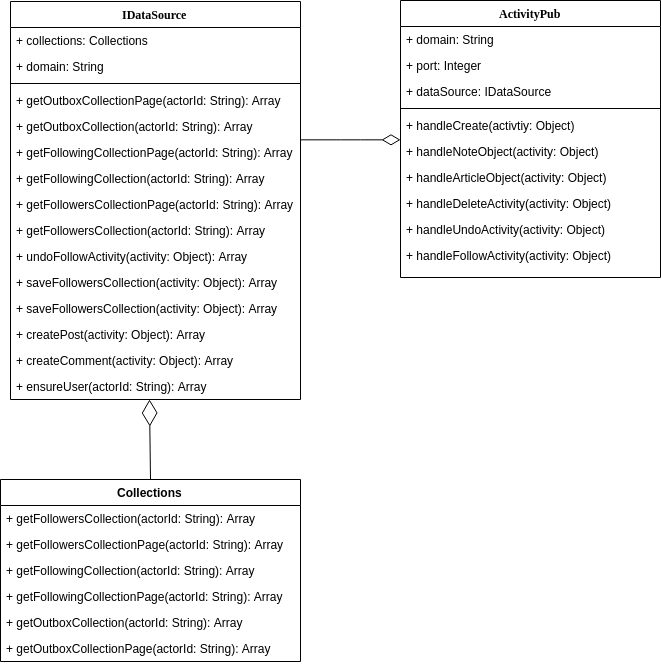
\includegraphics[scale=0.5]{figures/klassendiagramm-activitypub.png}
		\label{klassendiagramm-activitypub}
		\caption{Hauptkomponenten des förderierten Servers}
	\end{minipage}
\end{figure}

In der obigen Abbildung ist zu sehen, dass die \glqq Collections\grqq~Klasse Methoden enthält die zum Abruf von Sammlungen wie z. B. der \glqq Outbox Collection\grqq~benötigt werden. Sie dient lediglich der Weiterleitung von Aufrufen zur \glqq IDataSource\grqq~Klasse.\\

Haupteinstieg für die Express Middleware ist eine an jede Anfrage gehängte Klasse namens ActivityPub. Diese enthält eine statische \glqq \textit{init}\grqq~Methode zum initialisieren des ActivityPub Service. Darin wird, bei der alleinstehenden Version, ein eigener Express Server gestartet; Bei der integrierten Version wird ein Server Objekt mit frei zugänglichem Express Server erwartet um die Router Middleware hinzuzufügen.\\

\section{Server-zu-Server Protokoll}
